\documentclass[a4paper]{article}
\usepackage[T1]{fontenc}			% \chapter package
\usepackage[english]{babel}
\usepackage[english]{isodate}  		% date format
\usepackage{graphicx}				% manage images
\usepackage{amsfonts}
\usepackage{booktabs}				% high quality tables
\usepackage{amsmath}				% math package
\usepackage{amssymb}				% another math package (e.g. \nexists)
\usepackage{bm}                     % bold math symbols
\usepackage{mathtools}				% emphasize equations
\usepackage{stmaryrd} 				% '\llbracket' and '\rrbracket'
\usepackage{amsthm}					% better theorems
\usepackage{enumitem}				% manage list
\usepackage{pifont}					% nice itemize
\usepackage{cancel}					% cancel math equations
\usepackage{caption}				% custom caption
\usepackage[]{mdframed}				% box text
\usepackage{multirow}				% more lines in a table
\usepackage{textcomp, gensymb}		% degree symbol
\usepackage[x11names]{xcolor}		% RGB color
\usepackage[many]{tcolorbox}		% colorful box
\usepackage{multicol}				% more rows in a table (used for the lists)
\usepackage{listings}
\usepackage{url}
\usepackage{qrcode}
\usepackage{fontawesome5}
\usepackage{ragged2e}
\usepackage{cite}                   % references
\usepackage{imakeidx}               % index
\makeindex[program=makeindex, columns=1,
           title=Index, 
           intoc,
           options={-s index-style.ist}]
\usepackage{fancyhdr}

%\pdfcompresslevel=0
%\pdfobjcompresslevel=0

\definecolor{codegreen}{rgb}{0,0.6,0}
\definecolor{codegray}{rgb}{0.5,0.5,0.5}
\definecolor{codepurple}{rgb}{0.58,0,0.82}
\definecolor{backcolour}{rgb}{0.95,0.95,0.92}
\lstdefinestyle{mystyle}{
    backgroundcolor=\color{backcolour},
    commentstyle=\color{codegreen},
    keywordstyle=\color{magenta},
    numberstyle=\tiny\color{codegray},
    stringstyle=\color{codepurple},
    basicstyle=\ttfamily\footnotesize,
    breakatwhitespace=false,
    breaklines=true,
    captionpos=b,
    keepspaces=true,
    numbers=left,
    numbersep=5pt,
    showspaces=false,
    showstringspaces=false,
    showtabs=false,
    tabsize=2
}
\lstset{style=mystyle}


% thanks Mico: https://tex.stackexchange.com/a/60218/312896
\makeatletter
\renewcommand\paragraph{\@startsection{paragraph}{4}{\z@}%
            {-2.5ex\@plus -1ex \@minus -.25ex}%
            {1.25ex \@plus .25ex}%
            {\normalfont\normalsize\bfseries}}
\makeatother
\setcounter{secnumdepth}{4} % how many sectioning levels to assign numbers to
\setcounter{tocdepth}{4}    % how many sectioning levels to show in ToC


% draw a frame around given text
\newcommand{\framedtext}[1]{%
	\par%
	\noindent\fbox{%
		\parbox{\dimexpr\linewidth-2\fboxsep-2\fboxrule}{#1}%
	}%
}


% table of content links
\usepackage{xcolor}
\usepackage[linkcolor=black, citecolor=blue, urlcolor=cyan]{hyperref} % hypertexnames=false
\hypersetup{
	colorlinks=true
}


\newtheorem{theorem}{\textcolor{Red3}{\underline{Theorem}}}
\renewcommand{\qedsymbol}{QED}
\newcommand{\dquotes}[1]{``#1''}
\newcommand{\longline}{\noindent\rule{\textwidth}{0.4pt}}
\newcommand{\circledtext}[1]{\raisebox{.5pt}{\textcircled{\raisebox{-.9pt}{#1}}}}
\newcommand{\definition}[1]{\textcolor{Red3}{\textbf{#1}}\index{#1}}
\newcommand{\example}[1]{\textcolor{Green4}{\textbf{#1}}}
\newcommand{\highspace}{\vspace{1.2em}\noindent}
\newcommand{\version}{v0.2.0}


\begin{document}
    \newcounter{definition}[section]
    \newcounter{example}[section]
    \newcounter{exercise}[section]
    
    \newtcolorbox[use counter = definition]{definitionbox}[1][]{%
        breakable,
        enhanced,
        colback=red!5!white,
        colframe=red!75!black,
        fonttitle=\bfseries,
        title={Definition \thetcbcounter#1} %
    }

    \newtcolorbox[use counter = exercise]{exercisebox}[1][]{%
        breakable,
        enhanced,
        colback=Red3!5!white,
        colframe=Red3!75!black,
        fonttitle=\bfseries,
        title={Exercise \thetcbcounter#1} %
    }
    
    \newtcolorbox[use counter = example]{examplebox}[1][]{%
        breakable,
        enhanced,
        colback=Green4!5!white,
        colframe=Green4!75!black,
        fonttitle=\bfseries,
        title={Example \thetcbcounter#1} %
    }

    \newtcolorbox[]{deepeningbox}[1][]{%
        breakable,
        enhanced,
        colback=DarkOrange3!5!white,
        colframe=DarkOrange3!75!black,
        fonttitle=\bfseries,
        title={Deepening#1} %
    }

    %%%%%%%%%%%%%%%
    % Notes cover %
    %%%%%%%%%%%%%%%
    \author{260236}
\title{Parallel Computing - Notes - \version}
\date{\printdayoff\today}
\maketitle

    %%%%%%%%%%%
    % Preface %
    %%%%%%%%%%%
	\section*{Preface}

Every theory section in these notes has been taken from the sources:
\begin{itemize}
    \item Course slides.\cite{numerical-linear-algebra-polimi}
\end{itemize}
About:
\begin{itemize}
    \item[\faIcon{github}] \href{https://github.com/PoliMI-HPC-E-notes-projects-AndreVale69/HPC-E-PoliMI-university-notes}{GitHub repository}
    \begin{center}
        \qrcode{https://github.com/PoliMI-HPC-E-notes-projects-AndreVale69/HPC-E-PoliMI-university-notes}
    \end{center}
\end{itemize}
These notes are an unofficial resource and shouldn't replace the course material or any other book on numerical linear algebra. It is not made for commercial purposes. I've made the following notes to help me improve my knowledge and maybe it can be helpful for everyone.

As I have highlighted, a student should choose the teacher's material or a book on the topic. These notes can only be a helpful material.

\highspace

\subsection*{Correlated Projects}

During the Numerical Linear Algebra for HPC course, I was part of a team where we created a project that included two challenges related to the course. See more details in the corresponding repository:
\begin{itemize}
    \item[\faIcon{github}] \href{https://github.com/PoliMI-HPC-E-notes-projects-AndreVale69/NLA-challenges}{GitHub repository}
    \begin{center}
        \qrcode{https://github.com/PoliMI-HPC-E-notes-projects-AndreVale69/NLA-challenges}
    \end{center}
\end{itemize}

    %%%%%%%%%%%%%%%%%%%%%
    % Table of contents %
    %%%%%%%%%%%%%%%%%%%%%
    \tableofcontents
    \newpage

    %%%%%%%%%%%%%%%%%%%
    % Fancy pagestyle %
    %%%%%%%%%%%%%%%%%%%
    \pagestyle{fancy}
    \fancyhead{} % clear all header fields
    \fancyhead[R]{\nouppercase{\leftmark\hfill\rightmark}}

    %%%%%%%%%%%%%%%%%%
    % Basic Concepts %
    %%%%%%%%%%%%%%%%%%
    \section{Basic Concepts}

In this course, we introduce numerical methods for the solution of \textbf{Partial Differential Equations} (PDEs), with focus on the \textbf{Finite Element} (FE) \textbf{method}\footnote{The finite element method (FEM) is a popular method for numerically solving differential equations arising in engineering and mathematical modeling. Typical problem areas of interest include the traditional fields of structural analysis, heat transfer, fluid flow, mass transport, and electromagnetic potential. Computers are usually used to perform the calculations required. With high-speed supercomputers, better solutions can be achieved, and are often required to solve the largest and most complex problems. (\href{https://en.wikipedia.org/wiki/Finite_element_method}{source})} and the use of the computer for the construction of the PDEs numerical solution.

\highspace
We will consider the numerical approximation of elliptic and parabolic PDEs by considering their variational formulation, Galërkin and FE approximations in 1D/2D/3D, the theoretical properties and practical use of the methods, algorithmic aspects, and interpretation of the numerical results.

\highspace
Advanced topics include the approximation of saddle-point PDEs (Stokes equations), vectorial, nonlinear, and multiphysics differential problems, domain decomposition methods exploiting the properties of the PDEs, and the introduction to parallel computing for the FE method, i.e., in the \emph{High Performance Computing} (HPC) framework.

\highspace
Finally, the course will feature the use of the \href{https://www.dealii.org/}{\texttt{deal.II} software library}, a C++ open source FE library, and \href{https://www.paraview.org/}{ParaView} for the visualization of numerical solution and scientific computing data.

\newpage

\subsection{Mathematical Models and Scientific Computing}

\begin{definitionbox}[: Mathematical Model]
    A \definition{Mathematical Model} is a \textbf{set of} (algebraic or differential) \textbf{equations that is able to represent the features of a complex system or process}.

    \begin{flushleft}
        \textcolor{Green3}{\faIcon{question-circle} \textbf{Why do they exist?}}
    \end{flushleft}
    Models are \textbf{developed} to:
    \begin{itemize}
        \item Describe
        \item Forecast
        \item Control
    \end{itemize}
    The \textbf{behavior or evolution of such systems}.
\end{definitionbox}

\highspace
We are interested in the physics models. \textbf{Physics-based models} are those \textbf{mathematical models that are derived from physical principles} (like conservation laws of mass, momentum, energy, etc.) \textbf{and that encode natural laws of leading to (differential) equations whose solutions are often represented in the form of functions}. However, the analytical solution of such models is rarely available in closed form, for which numerical approximation methods are instead employed.

\highspace
\begin{definitionbox}[: Numerical Modelling]
    \definition{Numerical Modelling} indicates \textbf{sets of numerical methods that determine an approximate solution of the original} (often infinite-dimensional) \textbf{mathematical model}, by turing it into a \emph{discrete problem} (algebraic, finite-dimensional), whose dimension (size) is typically very large.
\end{definitionbox}

\highspace
\begin{definitionbox}[: Scientific Computing]
    \definition{Scientific Computing} is \textbf{a branch} of Mathematics \textbf{that numerically solves} (differential) \textbf{mathematical models by building approximate solutions though the use of a calculator}.
\end{definitionbox}

\highspace
For numerical models of large size, parallel architectures for calculators and the HPC framework are typically used.

\newpage

\begin{flushleft}
    \textcolor{Green3}{\faIcon{question-circle} \textbf{Why did we introduce mathematical models and physical models?}}
\end{flushleft}
Because they are connected and used together. Mathematical models are conventionally used altogether with theoretical (mathematical) models and experimental tests. Unfortunately, in several cases theoretical models are not available (like in Computational Medicine) or experimental tests are not meaningful or cannot be performed (for example, for nuclear testing). Physics-based models have witnessed an increasing role in the modern society in virtue of the massive developments of Scientific Computing and computational tools.

\highspace
Since a large amount of data is becoming available from multiple sources nowadays, data-driven models are fundamentals. \textbf{Data-driven models} are those mathematical models built from meaningful data that do not rely on physical principles, because the latter are not available or are not reliable, and whose construction calls for statical learning methods.

\highspace
Physics-based mathematical models (\textbf{mathematical problems}) are a fundamental pillar in the understanding and prediction of several physical phenomena and processes (\textbf{physical problems}). However, these mathematical models lead to problems that can rarely be solved analytically, or in an exact way (\textbf{exact solution}), especially for PDEs: with only a few exceptions, it is not possible to write their solution explicitly.

\highspace
Numerical methods and numerical approximation techniques (\textbf{numerical problems}) serve the purpose to determine an \textbf{approximate solution} of a mathematical model. When the calculator is used to determine such approximate solution, the latter is called \textbf{numerical solution} (see the Figure \ref{fig: scientific computing}).

\begin{figure}[!htp]
    \centering
    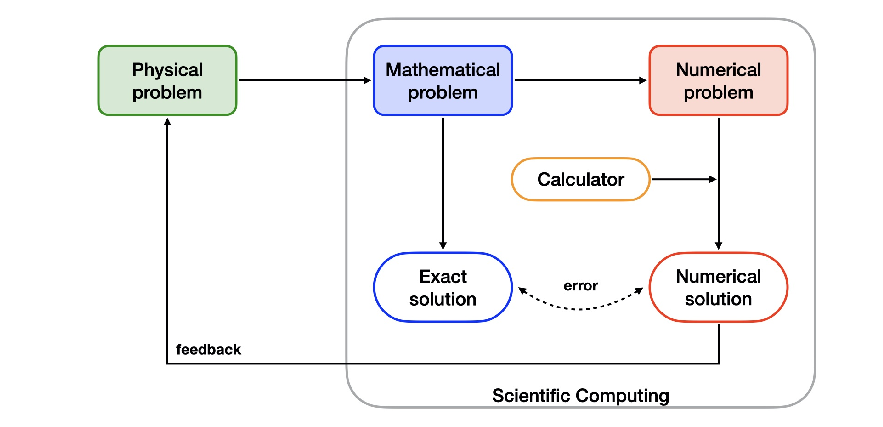
\includegraphics[width=\textwidth]{img/models-1.pdf}
    \caption{Scientific Computing.}
    \label{fig: scientific computing}
\end{figure}
    \subsection{Differential Models and PDEs}

\begin{definitionbox}[: Partial Differential Equation (PDE)]
    A \textbf{differential equation} (model) is an equation that involves \textbf{one or more derivatives of an unknown function}. In an \textbf{Ordinary Differential Equation} (ODE), \textbf{every derivative of the unknown solution is with respect to a single independent variable}. If instead, derivatives are partial, then we have a \definition{Partial Differential Equation (PDE)}.
\end{definitionbox}

\noindent
In other words, it is a differential equation where its derivatives are partial.

\highspace
There are different types of PDEs, and their nature depends on the conditions and their type. Mathematically, we can represent a \textbf{differential model} (equation) as follows:
\begin{equation}
    \mathcal{P}\left(u; g\right) = 0 \hspace{2em} \text{differential equation (mathematical problem)}
\end{equation}
Where:
\begin{itemize}
    \item $\mathcal{P}$ indicates the \emph{\textbf{model}};
    \item $u$ is the \emph{\textbf{exact solution}}, a function of one or more independent variables (space and/or time variables);
    \item $g$ indicates the \emph{\textbf{data}}.
\end{itemize}

\newpage

\subsubsection{ODEs}

\definition{Ordinary Differential Equation (ODE)} is also known as \textbf{initial value problem}.\index{Initial value problem}

\highspace
\begin{flushleft}
    \textcolor{Green3}{\faIcon{book} \textbf{I\textdegree ODE - Cauchy problem}}
\end{flushleft}
A \textbf{first order} ODE, a \textbf{Cauchy problem}, is a differential problem, whose:
\begin{itemize}
    \item \textbf{\emph{Solution}} $u = u\left(t\right)$ is a function of a single independent variable $t$, often interpreted as time.
    \item A \textbf{\emph{single condition}} is assigned on the solution, at a point (usually, the left end of the integration interval).
\end{itemize}
Its form is the following find $u : I \subset \mathbb{R} \rightarrow \mathbb{R}$ such that:
\begin{equation}
    \begin{cases}
        \dfrac{\mathrm{d}u}{\mathrm{d}t}\left(t\right) = f\left(t, u\left(t\right)\right) & t \in I \vspace{1em} \\
        u\left(t_{0}\right) = u_{0}
    \end{cases}
\end{equation}
Where:
\begin{itemize}
    \item $I = \left( t_{0}, t_{f} \right] \subset \mathbb{R}$ is a \emph{\textbf{time interval}};
    \item $u_{0}$ is the \emph{\textbf{initial value}} assigned at $t = t_{0}$;
    \item $f: I \times \mathbb{R} \rightarrow \mathbb{R}$
\end{itemize}
\textcolor{Green3}{\faIcon{question-circle} \textbf{Meaning}}. The equation describes the \textbf{evolution of a scalar quantity $u$ over time $t$}, \textbf{without distribution in space}.

\highspace
\textcolor{Green3}{\faIcon{question-circle} \textbf{Vectorial problems}}. In vectorial problems, the \textbf{unknown is a vector-valued function} $\mathbf{u} = \mathbf{u}\left(t\right)$, where $\mathbf{u} = \left(u_{1}, \dots, u_{m}\right) \in \mathbb{R}^{m}$, with $m \ge 1$. The first order Cauchy problem reads: find $\mathbf{u} : I \subset \mathbb{R} \rightarrow \mathbb{R}^{m}$ such that:
\begin{equation*}
    \begin{cases}
        \dfrac{\mathrm{d}\mathbf{u}}{\mathrm{d}t}\left(t\right) = \mathbf{f}\left(t, \mathbf{u}\left(t\right)\right) & t \in I \vspace{1em} \\
        \mathbf{u}\left(t_{0}\right) = \mathbf{u}_{0}
    \end{cases}
\end{equation*}
Where $\mathbf{u}_{0} \in \mathbb{R}^{m}$ is the initial datum and $\mathbf{f}: I \times \mathbb{R}^{m} \rightarrow \mathbb{R}^{m}$.

\highspace
\begin{flushleft}
    \textcolor{Green3}{\faIcon{book} \textbf{II\textdegree ODE - Cauchy problem}}
\end{flushleft}
A \textbf{second order Cauchy problem} sees second order time derivatives and two initial conditions. It reads as: find $u: I \subset \mathbb{R} \rightarrow \mathbb{R}$ such that:
\begin{equation}
    \begin{cases}
        \dfrac{\mathrm{d}^{2}u}{\mathrm{d}t^{2}}\left(t\right) = f\left(t, u\left(t\right), \dfrac{\mathrm{d}u}{\mathrm{d}t}\left(t\right)\right) & t \in I \vspace{1em} \\
        \dfrac{\mathrm{d}u}{\mathrm{d}t}\left(t_{0}\right) = v_{0} \vspace{1em} \\
        u\left(t_{0}\right) = u_{0}
    \end{cases}
\end{equation}
Where the initial data are $u_{0}$ and $v_{0}$, while $f: I \times \mathbb{R} \times \mathbb{R} \rightarrow \mathbb{R}$.
    \subsubsection{PDE, boundary value problem in 1D}

The \definition{Boundary value problem in 1D} is characterized by a \textbf{single independent variable} $x$, which represents the \textbf{space coordinate in an interval} $\Omega = \left(a,b\right) \in \mathbb{R}$ (1D).

\highspace
The problem involves \textbf{second order derivatives of the unknown solution} $u = u\left(x\right)$ with respect to $x$. The value of $u$, or the \textbf{value of its first derivate}, is a \textbf{set at the two boundaries of the domain} (interval) $\Omega$, that is at $x = a$ and $x = b$ (the domain boundary is $\partial\Omega = \left\{a,b\right\})$.

\highspace
Let us consider the following Poisson problem with (homogeneous) Dirichlet boundary conditions: find $u : \Omega \subset \mathbb{R} \rightarrow \mathbb{R}$ such that:
\begin{equation}
    \begin{cases}
        -\dfrac{\mathrm{d}^{2}u}{\mathrm{d}x^{2}}\left(x\right) = f\left(x\right) & x \in \Omega = \left(a,b\right) \vspace{1em} \\
        %
        u\left(a\right) = u\left(b\right) = 0
    \end{cases}
\end{equation}
This equation models a \textbf{stationary phenomenon} (the time variable doesn't appear in fact) and represent a \textbf{diffusion model}.

\highspace
\begin{examplebox}
    For example, the diffusion model models the diffusion of a pollutant along a 1D channel $\Omega = \left(a,b\right)$ or the vertical displacement of an \emph{elastic thread} fixed at its ends. In the first case, $f = f\left(x\right)$ indicates the source of the pollutant along the flow, while in the second case, $f$ is the traverse force acting on the elastic thread, in the hypothesis of negligible mass and small displacements of the thread.
\end{examplebox}

\noindent
\begin{flushleft}
    \textcolor{Green3}{\faIcon{balance-scale} \textbf{Boundary value problem in 1D vs ODE}}
\end{flushleft}
We remark that the \textbf{boundary value problem in 1D is a particular case of PDEs}, even if it involves only derivatives with respect to a single independent variable $x$. Indeed, even if apparently similar to a second order ODE, the boundary value problem is in reality substantially \textbf{different} from an ODE:
\begin{itemize}
    \item In ODE, two conditions are set at $t = t_{0}$;
    \item In the boundary value problem in 1D, one condition is set at $x = a$ and the other one at $x = b$.
\end{itemize}
The conditions in the boundary value problem determine to the so-called global nature of the model.
    \subsubsection{PDE, initial and boundary value problem in 1D}

\definition{Initial and boundary value problem in 1D} is a type of problems that concern equations that \textbf{depend on space and time}:
\begin{itemize}
    \item The \textbf{unknown solution} $u = u\left(x,t\right)$ both depends on the space coordinate $x \in \Omega \subset \mathbb{R}$ in 1D;
    
    \item The \textbf{time variable} $t \in I \subset I$.
\end{itemize}
In this case, the initial conditions at $t = 0$ must be prescribed, as well as the boundary conditions at the ends of the interval in 1D.

\highspace
The \definition{Heat equation}, also known as \definition{Diffusion equation}, with Dirichlet boundary conditions assumes the following form: find $u: \Omega \times I \rightarrow \mathbb{R}$ such that:
\begin{equation}
    \begin{cases}
        \dfrac{\partial u}{\partial t}\left(x,t\right) - \mu \dfrac{\partial^{2}u}{\partial x^{2}}\left(x,t\right) = f\left(x,t\right) & x \in \Omega = \left(a,b\right), t \in I \vspace{1em} \\
        %
        u\left(a,t\right) = u\left(b,t\right) = 0 & t \in I \\
        %
        u\left(x, t_{0}\right) = u_{0}\left(x\right) & x \in \Omega = \left(a,b\right)
    \end{cases}
\end{equation}

\begin{examplebox}
    For example, the unknown function $u \left(x,t\right)$ describes the temperature in a point $x \in \Omega = \left(a,b\right)$ and time $t \in I$ of a metallic bar covering the space interval $\Omega$. The diffusion coefficient $\mu$ represents the thermal response of the material and it is related to its thermal conductivity. The Dirichlet boundary conditions express the fact that the ends of the bar are kept at a reference temperature (zero degrees in this case), while at time $t = t_{0}$ the temperature is assigned in each point $x \in \Omega$ through the initial function $u_{0}\left(x\right)$. Finally, the bar is subject to a heat source of linear density $f\left(x,t\right)$.
\end{examplebox}
    \subsubsection{PDE, boundary value problem in multidimensional domains}

The Poisson problem (equation \ref{eq: Poisson problem}, page \pageref{eq: Poisson problem}) can be \textbf{extended in multidimensional domains} $\Omega \subset \mathbb{R}^{d}$, with $d = 2, 3$; the solution is $u = u\left(\mathbf{x}\right)$, where $\mathbf{x} = \left(x_{1}, \dots, x_{d}\right)^{T} \in \mathbb{R}^{d}$. This leads to the following Poisson problem with (homogeneous) Dirichlet boundary conditions: find $u: \Omega \subset \mathbb{R}^{d} \rightarrow \mathbb{R}$ such that:
\begin{equation}
    \begin{cases}
        -\Delta u = f   & \text{in } \Omega \: \left(\text{i.e. } \mathbf{x} \in \Omega\right) \\
        u = 0           & \text{on } \partial\Omega \: \left(\text{i.e. } \mathbf{x} \in \partial\Omega\right)
    \end{cases}
\end{equation}
Where:
\begin{itemize}
    \item The \definition{Laplace operator}:
    \begin{equation*}
        \Delta u \left(\mathbf{x}\right) := \displaystyle\sum_{i=1}^{d} \dfrac{\partial^{2} u}{\partial x_{i}^{2}}\left(\mathbf{x}\right)
    \end{equation*}

    \item The \textbf{domain} $\Omega \subset \mathbb{R}^{d}$ is endowed with boundary $\partial \Omega$;

    \item $f = f\left(x\right)$ is the \emph{\textbf{external forcing term}}.
\end{itemize}
This equation is used \example{for example} to \textbf{model the vertical displacement of an elastic membrane fixed at the boundaries}.
    \subsubsection{Classification of PDEs}

A PDE is a relationship among:
\begin{itemize}
    \item The partial derivatives of a function $u = u\left(\mathbf{u}, t\right)$, that is the PDE \textbf{solution};
    \item \textbf{Spatial coordinates} $\mathbf{x} = \left(x_{1}, \dots, x_{d}\right)^{T} \in \mathbb{R}^{d}$ on which the solution depends (if the problem is defined in a spatial domain $\Omega \subset \mathbb{R}^{d}$).
    \item \textbf{Time variable} $t$.
\end{itemize}
Therefore, a PDE can be written as:
\begin{equation}
    \mathcal{P}\left(
        u,
        \dfrac{\partial u}{\partial t},
        \dfrac{\partial u}{\partial x_{1}},
        \dots,
        \dfrac{\partial u}{\partial x_{d}},
        \dots,
        \dfrac{\partial^{p_{1} + \dots + p_{d} + p_{t}} u}{\partial x_{1}^{p_{1}} \dots \partial x_{d}^{p_{d}} \: \partial t^{p_{t}}},
        \mathbf{x},
        t;
        g
    \right) = 0
\end{equation}
Where $p_{1}, \dots, p_{d}, p_{t} \in \mathbb{N}$ and $g$ are the data.

\highspace
\begin{definitionbox}[: PDE order]
    The \definition{PDE order} is the \textbf{maximum order of derivation} that appears in $\mathcal{P}$, that is:
    \begin{equation}
        q = p_{1} + \dots + p_{d} + p_{t}
    \end{equation}
\end{definitionbox}

\begin{definitionbox}[: PDE is linear]
    The \definition{PDE is linear} if $\mathcal{P}$ \textbf{linearly depends} on $u$ and its \textbf{derivatives}.
\end{definitionbox}

\highspace
\begin{flushleft}
    \textcolor{Green3}{\faIcon{square-root-alt} \textbf{Classification}}
\end{flushleft}
Let us focus on linear PDEs of order $q = 2$ with constant coefficients, so that the general PDE formulation is:
\begin{equation*}
    \mathcal{L}u = g
\end{equation*}
Where $\mathcal{L}$ is a second order, \textbf{linear differential operator}. When only two independent variables (our case) $x_{1}$ and $x_{2}$ are considered, the operator $\mathcal{L}$ applied to the function $u$ reads:
\begin{equation*}
    \mathcal{L}u = 
    A \cdot \dfrac{\partial^{2} u}{\partial x_{1}^{2}} +
    B \cdot \dfrac{\partial^{2} u}{\partial x_{1} \: \partial x_{2}} +
    C \cdot \dfrac{\partial^{2} u}{\partial x_{2}^{2}} +
    D \cdot \dfrac{\partial u}{\partial x_{1}} +
    E \cdot \dfrac{\partial u}{\partial x_{2}} +
    F \cdot u
\end{equation*}
For some constant coefficients $A, B, C, D, E, F, G \in \mathbb{R}$. If $d = 2$ (our case), the \textbf{independent variables} can represent the \emph{space coordinates}:
\begin{itemize}
    \item $x_{1} = x$
    \item $x_{2} = y$
\end{itemize}
After introducing the \definition{PDE discriminant} (a quantity that helps determine the type of PDE):
\begin{equation}
   \Delta := B^{2} - 4AC 
\end{equation}
\newpage
\noindent
The PDE can be classified as:
\begin{itemize}
    \item \definition{Elliptic PDE} if $\Delta < 0$
    \item \definition{Parabolic PDE} if $\Delta = 0$
    \item \definition{Hyperbolic PDE} if $\Delta > 0$
\end{itemize}

\begin{flushleft}
    \textcolor{Green3}{\faIcon{question-circle} \textbf{What are the implications of PDE classification?}}
\end{flushleft}
The different nature of the PDE impacts on:
\begin{itemize}
    \item \textbf{Type} and \textbf{amount of data to prescribe as boundary};
    \item \textbf{Initial conditions} to ensure the well-posedness of the problem (existence and uniqueness of the solution);
    \item The \textbf{phenomena that can be described} by the PDE;
    \item The \textbf{information that encapsulates}.
\end{itemize}
In general:
\begin{itemize}
    \item \textbf{Elliptic PDE} typically describes \textbf{stationary phenomena}, without time evolution of quantities.
    \item \textbf{Parabolic PDE} describes \textbf{wave propagation phenomena} with \underline{infinite} velocity of propagation.
    \item \textbf{Hyperbolic PDE} describes \textbf{wave propagation phenomena} but with \underline{finite} velocity of propagation.
\end{itemize}
    \subsection{Numerical Methods}

Since in most cases of practical interest we \textbf{cannot solve a PDE analytically}, we need to use \textbf{numerical methods} that allow us to construct an \emph{approximation} $u_{h}$ of the \emph{exact solution} $u$, for which the corresponding \emph{error} $\left(u - u_{h}\right)$ can be quantified and/or estimated.
\begin{equation*}
    \begin{array}{cc}
        \mathcal{P}\left(u; g\right) = 0 \hspace{1em} & \text{PDE (mathematical problem)} \\ [.3em]
        \downarrow \hspace{1em} & \emph{numerical method} \\ [.3em]
        \mathcal{P}_{h}\left(u_{h}; g_{h}\right) = 0 \hspace{1em} & \text{approximate PDE (numerical problem)}
    \end{array}
\end{equation*}
Where:
\begin{itemize}
    \item $g_{h}$ is an approximation of the data $g$;
    \item $\mathcal{P}_{h}$ is a characterization of the approximate problem.
\end{itemize}
The subscript $h$ indicates a \textbf{discretization parameter} that characterizes the numerical approximation. Conventionally, the smaller is $h$, the better is the approximation of $u$ made by $u_{h}$. Furthermore, the error $\left(u - u_{h}\right)$ tends to zero as $h$ gets smaller and smaller. In this course, we will specifically introduce the FE method (page \pageref{definition: Finite Element Method (FEM)}) to build the numerical approximation of PDEs.

\highspace
\begin{flushleft}
    \textcolor{Green3}{\faIcon{bookmark} \textbf{Summary Notation}}
\end{flushleft}

\begin{table}[!htp]
    \centering
    \begin{tabular}{@{} c p{25em} @{}}
        \toprule
        \textbf{Notation} & \textbf{Description} \\
        \midrule
        $\mathcal{P}\left(u; g\right) = 0$ & PDE (mathematical problem) \\ [.5em]
        $u$ & \textbf{\emph{exact solution}} of a PDE \\ [.5em]
        $u_{h}$ & \textbf{\emph{approximate solution}} of a PDE \\ [.5em]
        $\left(u - u_{h}\right)$ & \textbf{\emph{error}} (quantified and/or estimated; tends to zero if $h$ is smaller) \\ [.5em]
        $h$ & \textbf{\emph{discretization parameter}} ($\downarrow$ smaller $h$, better approximation; $\uparrow$ higher $h$, poor approximation) \\ [.5em]
        $\mathcal{P}_{h}\left(u_{h}; g_{h}\right) = 0$ & approximate PDE (numerical problem) \\ [.5em]
        $g_{h}$ & \textbf{\emph{approximation}} of the \textbf{\emph{data}} $g$ \\ [.5em]
        $\mathcal{P}_{h}$ & \textbf{\emph{characterization}} of the approximate problem. \\
        \bottomrule
    \end{tabular}
    \caption{Notation used to approximate the PDE with numerical methods.}
\end{table}
    \subsection{From Mathematical to Numerical Problem}

\subsubsection{The mathematical problem}

Let us consider a \definition{Physical Problem (PP)} endowed with a \textbf{physical solution}, let say $u_{ph}$, and \textbf{dependent on data} indicated with $g$.

\highspace
The \definition{Mathematical Problem (MP)} is represented by the \textbf{mathematical formulation of the PP} and has \textbf{mathematical solution} $u$. Therefore, we indicate the MP as:
\begin{equation}\label{eq: mathematical problem}
    \mathcal{P}\left(u; g\right) = 0
\end{equation}
Where:
\begin{itemize}
    \item $u \in \mathcal{U}$
    \item $g \in \mathcal{G}$, and $\mathcal{G}$ is the set or space of \textbf{admissible data}.
\end{itemize}
Where $\mathcal{U}$ and $\mathcal{G}$ are suitable sets or spaces.

\highspace
\begin{definitionbox}[: Model Error]
    The error between the physical and mathematical solutions is called \definition{Model Error}:
    \begin{equation}
        e_{m} := u_{ph} - u
    \end{equation}
    Where:
    \begin{itemize}
        \item $u_{ph}$ is the physical solution;
        \item $u$ is the mathematical solution.
    \end{itemize}
\end{definitionbox}

\noindent
The model error takes into account all those \textbf{characteristics of the PP that are not represented or captured by the MP}.

\highspace
\begin{flushleft}
    \textcolor{Green3}{\faIcon{question-circle} \textbf{When a Mathematical Problem is \emph{well-posed}?}}
\end{flushleft}
\begin{definitionbox}[: well-posed MP]
    The mathematical problem MP is \emph{well-posed} (\textbf{stable}) if and only if there \textbf{exists a unique solution} $u \in \mathcal{U}$ \textbf{that continuously depend on the data} $g \in \mathcal{G}$.
\end{definitionbox}

\noindent
From the previous definition, we remark that $\mathcal{G}$ is the set of admissible data, i.e., those for which the MP admits a unique solution. Furthermore, \emph{continuously depend on the data} means that \textbf{small perturbations on data} $g \in \mathcal{G}$ \textbf{lead to small changes on the solution} $u \in \mathcal{U}$ of the MP. However, a measure of this sensitivity is given by the condition number of the MP.
    \subsubsection{The Numerical Problem (NP)}

The \definition{Numerical Problem (NP)} is an \textbf{approximation of the Mathematical Problem} (MP, equation \ref{eq: mathematical problem (MP)}, page \pageref{eq: mathematical problem (MP)}). We indicate its \textbf{numerical solution} as $u_{h}$, where $h$ stands as a suitable \textbf{discretization parameter}.
\begin{equation}\label{eq: numerical problem (NP)}
    \mathcal{P}_{h}\left(u_{h}; g_{h}\right) = 0
\end{equation}
Where:
\begin{itemize}
    \item $u_{h} \in \mathcal{U}_{h}$
    \item $g_{h} \in \mathcal{G}_{h}$, and $g_{h}$ is the representation of the \textbf{data in the NP}.
\end{itemize}
Where $\mathcal{U}_{h}$ and $\mathcal{G}_{h}$ are suitable sets or spaces.

\highspace
\begin{definitionbox}[: Truncation Error]
    The error between the mathematical and numerical solutions is called \definition{Truncation Error}:
    \begin{equation}\label{eq: Truncation Error}
        e_{h} := u - u_{h}
    \end{equation}
    Where:
    \begin{itemize}
        \item $u$ is the mathematical solution;
        \item $u_{h}$ is the numerical solution.
    \end{itemize}
\end{definitionbox}

\noindent
The truncation error can be considered as the error resulting from the \textbf{discretization of the MP}.

\highspace
\begin{flushleft}
    \textcolor{Green3}{\faIcon{laptop-code} \textbf{Numerical solution calculated on the computer}}
\end{flushleft}
When the numerical solution is computed by running the algorithm on a computer, we need more notations and concepts.
\begin{itemize}
    \item $\widehat{u}_{h}$ is the \textbf{final solution}.

    \item The final solution is affected by a \definition{Round-Off error} $e_{r}$:
    \begin{equation}\label{eq: Round-Off error}
        e_{r} := u_{h} - \widehat{u}_{h}
    \end{equation}
    Such round-off errors depend on the machine architecture, on the representation of the numbers at the calculator, and on operations made in floating-point arithmetic.

    \item The truncation error $e_{h}$ (equation \ref{eq: Truncation Error}, page \pageref{eq: Truncation Error}) and the Round-Off error $e_{r}$ (equation \ref{eq: Round-Off error}) concur to determine the \definition{Computational error} $e_{c}$:
    \begin{equation}
        e_{c} := e_{h} + e_{r} = \left(u - \cancel{u_{h}}\right) + \left(\cancel{u_{h}} - \widehat{u}_{h}\right) = u - \widehat{u}_{h}
    \end{equation}
    For some NP, we can have a round-off error less than a truncation error $\left|e_{r}\right| \ll \left|e_{h}\right|$, for which $e_{c} \approx e_{h}$.
\end{itemize}

\newpage

\begin{flushleft}
    \textcolor{Green3}{\faIcon{question-circle} \textbf{When a Numerical Problem is \emph{well-posed}?}}
\end{flushleft}
\begin{definitionbox}[: \emph{well-posed} NP]
    The numerical problem NP is \emph{well-posed} (\textbf{stable}) if and only if there \textbf{exists a unique solution} $u_{h} \in \mathcal{U}_{h}$ \textbf{that continuously depends on the data} $g_{h} \in \mathcal{G}_{h}$.
\end{definitionbox}

\highspace
\begin{flushleft}
    \textcolor{Green3}{\faIcon{laptop-code} \textbf{Consider the numerical solution calculated only on the computer}}
\end{flushleft}
In practice, numerical solutions are computed on a computer. Therefore, it is reasonable to obtain a computational error that tends to zero as the numerical method improves, namely as the discretization parameter $h$ goes to zero. This concept is encoded in the definition of convergence.

\begin{definitionbox}[: \emph{convergence} NP]
    The NP is \textbf{convergent} when the \textbf{computational error tends to zero} for $h$ tending to zero, that is:
    \begin{equation}
        \lim\limits_{h \rightarrow 0} e_{c} = 0
    \end{equation}
\end{definitionbox}

\noindent
A crucial aspect is to qualify the convergence of the NP, that is determining the convergence order of the NP.

\begin{definitionbox}[: convergence order]\index{Convergence order}
    If $\left|e_{c}\right| \le Ch^{p}$, with $C$ a positive constant independent of $h$ and $p$, then the NP is \textbf{convergent with order} $p$.
\end{definitionbox}

\highspace
\begin{flushleft}
    \textcolor{Green3}{\faIcon{question-circle} \textbf{How to estimate the convergence order?}}
\end{flushleft}
The convergence order can be estimated for many reasons (error estimation, method comparison, accuracy verification, etc.). If there exists a constant $\tilde{C} \le C$ independent of $h$ and $p$ such that $\tilde{C}h^{p} \le \left|e_{c}\right| \le C h^{p}$, then we can write $\left|e_{c}\right| \approxeq Ch^{p}$ and we can \textbf{estimate the convergence order $p$ of the NP by using the known solution $u$ of the MP}. There are two approaches:
\begin{enumerate}
    \item \textbf{Algebraic estimation} of $p$.
    \begin{enumerate}
        \item We compute the computational errors $e_{c1}$ and $e_{c2}$ for the NP corresponding to two different values of $h$ that are \dquotes{sufficietly} small, say $h_{1}$ and $h_{2}$.
        \item Then:
        \begin{itemize}
            \item Writing $\left|e_{c1}\right| \approxeq Ch_{1}^{p}$ and $\left|e_{c2}\right| \approxeq Ch_{2}^{p}$
            \item Noticing that $\dfrac{\left|e_{c1}\right|}{\left|e_{c2}\right|} = \left(\dfrac{h_{1}}{h_{2}}\right)^{p}$
        \end{itemize}
        We estimate the order $p$ as:
        \begin{equation}
            p = \dfrac{
                \log\left(\dfrac{\left|e_{c1}\right|}{\left|e_{c2}\right|}\right)
            }{
                \log\left(\dfrac{h_{1}}{h_{2}}\right)
            }
        \end{equation}
    \end{enumerate}
    
    \item \textbf{Graphical estimation} of $p$. We represent the errors $\left|e_{c}\right|$ and $h$ on a plot in log-log scale. As $\log\left|e_{c}\right| = \log\left(Ch^{p}\right) = log\left(C\right) + p \log\left(h\right)$, we have $p = \arctan\left(\theta\right)$, where $\theta$ is the slope of the curve $\left(h, e_{c}\right)$, a straight line in log-log scale. Instead of computing $\theta$, it is possible to verify that the curves $\left(h, e_{c}\right)$ and $\left(h, h^{p}\right)$ are parallel in log-log scale.

    In other words it involves plotting the error against the step size on a log-log scale and analyzing the resulting graph:
    \begin{enumerate}
        \item \emph{\textbf{Compute Errors}}: Perform the numerical method for several step sizes $h$, such as $ h_{1}, h_{2}, h_{3}, \dots $, and compute the corresponding errors $ e_{1}, e_{2}, e_{3}, \dots $.

        \item \emph{\textbf{Log-Log Plot}}: Plot the errors $e_{i}$ against the step sizes $h_{i}$ on a log-log scale. This means we plot $\log\left(h_{i}\right)$ on the x-axis and $\log\left(e_{i}\right)$ on the y-axis.

        \item \emph{\textbf{Linear Relationship}}: If the method has a convergence order $p$, the relationship between the error and the step size should follow $e \approx C h^p $. Taking the logarithm of both sides gives:
        \begin{equation*}
            \log\left(e\right) \approx \log\left(C\right) + p \log\left(h\right)
        \end{equation*}
        This indicates that the plot of $\log\left(e\right)$ versus $\log\left(h\right)$ should be a straight line with a slope equal to $p$.

        \item \emph{\textbf{Determine Slope}}: The slope of the line in the log-log plot is the convergence order $p$. We can estimate this slope by fitting a linear regression line to the data points.
    \end{enumerate}

    \begin{figure}[!htp]
        \centering
        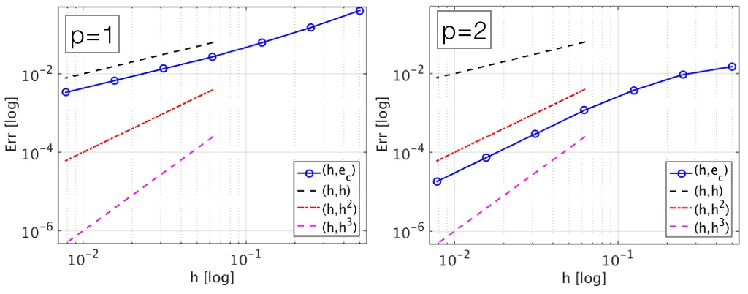
\includegraphics[width=\textwidth]{img/graphical-estimate-1.pdf}
        \caption{Graphical estimation of the convergence order $p$ of a NP: computational errors $\left|e_{c}\right|$ vs $h$.}
    \end{figure}
\end{enumerate}

\newpage

\begin{flushleft}
    \textcolor{Green3}{\faIcon{question-circle} \textbf{When is convergence guaranteed in NP?}}
\end{flushleft}
Unfortunately, a \textbf{\emph{well-posed} NP is not necessarily convergent}. To ensure convergence of the NP, this is required to satisfy the consistency property (roughly speaking, the NP must be a \dquotes{faithful copy} of the original MP).

\highspace
\begin{definitionbox}[: NP consisten and strongly consistent]
    The Numerical Problem NP is \textbf{consistent} if and only if:
    \begin{equation*}
        \lim\limits_{h \rightarrow 0}\mathcal{P}_{h}\left(u; g\right) = \mathcal{P}\left(u;g\right) = 0 \hspace{2em} g \in \mathcal{G}_{h}
    \end{equation*}

    The Numerical Problem NP is \textbf{\emph{strongly} consistent} if and only if:
    \begin{equation*}
        \mathcal{P}_{h}\left(u; g\right) \equiv \mathcal{P}\left(u;g\right) = 0 \hspace{2em} \forall h > 0, \: g \in \mathcal{G}_{h}
    \end{equation*}
\end{definitionbox}

\highspace
Let highlights the main differences:
\begin{itemize}
    \item Definition:
    \begin{itemize}
        \item \textcolor{Green4}{\emph{\textbf{Consistent}}}. Consistency requires that as the discretization parameter \( h \) tends to zero $\lim\limits_{h \rightarrow 0}$, the process \( \mathcal{P}_{h}(u; g) \) approaches the exact process \( \mathcal{P}(u; g) \) and both become zero. This means that \textbf{over time and with finer discretization}, the \textbf{numerical approximation converges to the exact solution}.

        \item \textcolor{Green4}{\emph{\textbf{Strongly Consistent}}}. Strong consistency means that for any positive value of \( h \) ($\forall h > 0$, no matter how small), the process \( \mathcal{P}_{h}(u; g) \) is exactly equal to the exact process \( \mathcal{P}(u; g) \) and both are zero. This implies that the \textbf{numerical approximation already matches the exact solution for any step size}.
    \end{itemize}

    \item Condition of $h$:
    \begin{itemize}
        \item \textcolor{Green4}{\emph{\textbf{Consistent}}}. The condition applies in the limit as \( h \) approaches zero. The \textbf{process gradually converges to the exact solution as the discretization parameter becomes infinitesimally small}.

        \item \textcolor{Green4}{\emph{\textbf{Strongly Consistent}}}. The condition applies for all \( h > 0 \). This is a \textbf{stronger requirement} because it demands that the numerical method is \textbf{accurate for any discretization parameter}, not just in the limit.
    \end{itemize}
\end{itemize}
In practice, the \emph{Consistent} indicates that the numerical method improves and approaches the exact solution as the discretization parameter is refined. It guarantees eventual \emph{\textbf{accuracy}}, \emph{\textbf{but not necessarily immediate or uniform accuracy for larger}} \( h \). On the other hand, \emph{Strongly Consistent} indicates that the numerical method is always accurate, regardless of the discretization parameter. This implies a \emph{\textbf{higher level of reliability and precision for any}} \( h \), making it a stronger and more robust form of consistency.

\newpage

\noindent
The \definition{Lax-Richtmyer Equivalence Theorem} is a cornerstone of numerical analysis, linking the concepts of consistency, well-posedness (stability), and convergence. It provides a \textbf{rigorous framework for validating numerical methods and ensuring that they produce accurate and reliable solutions}. Furthermore, the following theorem guarantees that if a \textbf{\emph{numerical problem is well-posed and consistent, then the NP is also convergent}}.
\begin{theorem}[Lax-Richtmyer, equivalence]
    If the Numerical Problem NP:
    \begin{equation*}
        \mathcal{P}_{h}\left(u_{h}; g_{h}\right) = 0 \hspace{2em} u_{h} \in \mathcal{U}_{h}, \: g_{h} \in \mathcal{G}_{h}
    \end{equation*}
    Is consistent:
    \begin{equation*}
        \lim\limits_{h \rightarrow 0}\mathcal{P}_{h}\left(u; g\right) = \mathcal{P}\left(u;g\right) = 0 \hspace{2em} g \in \mathcal{G}_{h}
    \end{equation*}
    Then, it is well-posed if and only if it is also convergent.
\end{theorem}

\noindent
It is a fundamental theorem in numerical analysis because \textbf{it ensures that stability and consistency are sufficient to guarantee convergence}. Conversely, if we have a proof that the NP is consistent, we \dquotes{only} need to show that the problem is well-posed to automatically prove convergence (and vice versa).

\highspace
\begin{figure}[!htp]
    \centering
    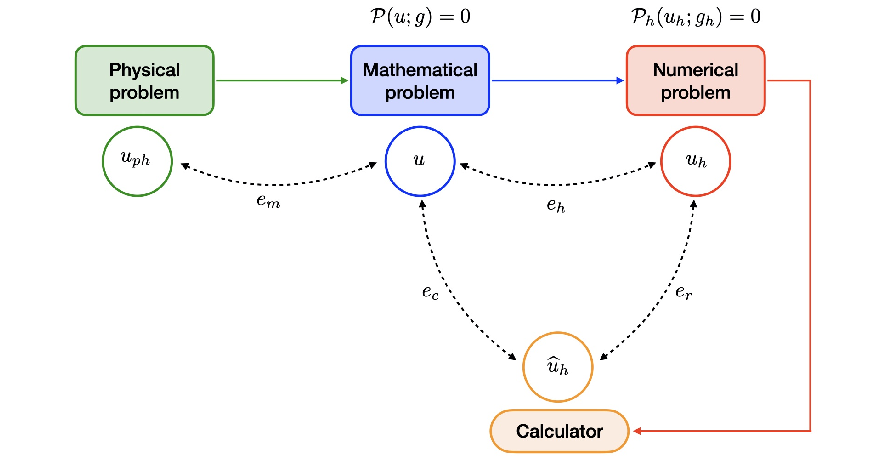
\includegraphics[width=\textwidth]{img/pp-mp-np-1.pdf}
    \caption{Physical (PP), Mathematical (MP), and Numerical (NP) problems. Corresponding solutions $\left(u_{ph}, u, u_{h}, \text{ and } \widehat{u}_{h}\right)$ and errors (model $e_{m} = u_{ph} - u$, truncation $e_{h} = u - u_{h}$, round-off $e_{r} = u_{h} - \widehat{u}_{h}$, and computational $e_{c} = e_{h} + e_{r}$ errors).}
    \label{fig: PP, MP and NP}
\end{figure}

    %%%%%%%%%%%%%%%%%%%%%%%%%%
    % Bibliography and index %
    %%%%%%%%%%%%%%%%%%%%%%%%%%
    \pagestyle{fancy}
\fancyhead{} % clear all header fields
\fancyhead[R]{\nouppercase{\leftmark}}

\bibliography{bibtex}{}
\bibliographystyle{plain}

\newpage

\printindex
\end{document}